\documentclass[a4paper]{llncs}
\usepackage[T1]{fontenc}
\usepackage[utf8]{inputenc}
\usepackage{authblk}
\usepackage{graphicx, epstopdf, color, setspace, algorithm, amsfonts, amsmath, mathtools, nicefrac}
\usepackage[algo2e, noend, noline, linesnumbered]{algorithm2e}
\SetKwIF{If}{ElseIf}{Else}{if}{then}{else if}{else}{endif}
\RestyleAlgo{boxruled}
\setlength{\textfloatsep}{.5cm}
\newcommand{\func}[1]{{\sc #1}}
\newcommand{\tuple}[1]{\ensuremath{\left \langle #1 \right \rangle }}
\DontPrintSemicolon
\DeclarePairedDelimiter{\ceil}{\lceil}{\rceil}
\DeclarePairedDelimiter{\floor}{\lfloor}{\rfloor}
\newcommand{\eg}{{\it e.g.,}~}
\newcommand{\ie}{{\it i.e.,}~}
\newcommand{\bE}{\mathbb{E}}
\newcommand{\cf}{{cf.}~}
\newcommand{\TODO}[1]{\textbf{\color{red}#1}}
\graphicspath{{img/}}
\pagestyle{headings}
\title{Minimizing~Simple~and~Cumulative~Regret in~Monte-Carlo~Tree~Search}

\author{Tom~Pepels\inst{1} \and Tristan~Cazenave\inst{2} \and
Mark~H.M.~Winands\inst{1} \and Marc~Lanctot\inst{1}}

\institute{Department of Knowledge Engineering,  Maastricht University\\ \email{\{tom.pepels,m.winands,marc.lanctot\}@maastrichtuniversity.nl} \and LAMSADE - Université Paris-Dauphine \\ \email{cazenave@lamsade.dauphine.fr}}

\begin{document}

\maketitle

% lanctot-edit: minor grammar + rephrasings of abstract
\begin{abstract} Regret minimization is key to both the Multi-Armed Bandit problem and Monte-Carlo Tree Search (MCTS). Recently, simple regret, \ie the regret of not recommending the best action, has been proposed as an alternative to cumulative regret in MCTS, \ie regret accumulated over time. Each type of regret is appropriate in different contexts. Although the majority of MCTS research applies the UCT selection policy for minimizing cumulative regret in the tree, this paper introduces a new MCTS variant, Hybrid MCTS (H-MCTS), which minimizes both types of regret in different parts of the tree. H-MCTS uses SHOT, a recursive version of Sequential Halving, to minimize simple regret near the root, and UCT when descending further down the tree. We discuss the theoretical foundation for this new search technique, and show the performance of H-MCTS in six distinct two-player games: Amazons, AtariGo, Ataxx, Breakthrough, NoGo, and Pentalath.

\end{abstract}

\section{Introduction}
\label{sec:intro}

%lanctot-edit:
%The Multi-Armed Bandit (MAB) problem is defined as a stochastic decision making problem~\cite{auer2002using}. An agent is faced with several options, each with their own reward distribution. Based on sampling the search space an agent is to select the option with the best reward distribution. 
% + minor rephrasings
The Multi-Armed Bandit (MAB) problem is a decision making problem~\cite{auer2002using} where an agent is faced with several options. On each time step, an agent selects one of the options and observes a reward drawn from some distribution. This process is then repeated for a number of time steps.
Generally the problem is described as choosing between the most rewarding arm of a multi-armed slot machine found in casinos. The agent can explore by pulling an arm and observing the resulting reward. The reward can be drawn from either a fixed or changing probability distribution. Each pull and the returned reward constitutes a sample. Algorithms used in MAB research have been developed to minimize \emph{cumulative regret}. Cumulative regret is the expected regret of not having sampled the single best option in hindsight. This type of regret is accumulated during execution of the algorithm, each time a non-optimal arm is sampled the cumulative regret increases. UCB1~\cite{auer2002using} is a selection policy for the MAB problem, which minimizes cumulative regret, converging to the empirically best arm. Once the best arm is found by exploring the available options, UCB1 exploits it by repeatedly sampling it, minimizing overall cumulative regret. This policy was adapted to be used in Monte-Carlo Tree Search (MCTS) in the form of UCT~\cite{kocsis2006bandit}.

Recently, \emph{simple regret} has been proposed as a new criterion for assessing the performance of both MAB~\cite{audibert2010best,Bubeck11Pure} and MCTS~\cite{Cazenave14SHOT,Feldman12BRUE,tolpin2012mcts} algorithms. Simple regret is defined as the expected error between an algorithm's recommendation, and the optimal decision. It is a naturally fitting quantity to optimize in the MCTS setting, because all simulations executed by MCTS are for the mere purpose of learning good moves. Moreover, the final move chosen after all simulations are performed, \ie the \emph{recommendation}, is the one that has real consequence. Nonetheless, since the introduction of Monte-Carlo Tree Search (MCTS)~\cite{kocsis2006bandit} and its subsequent adoption by games researchers UCT~\cite{kocsis2006bandit}, or some variant thereof, has become the ``default'' selection policy~(\cf~\cite{browne2012survey}). 

\vspace{2mm}
In this paper, we present a new, hybrid MCTS technique that utilizes both UCT, and Sequential Halving~\cite{Karnin13SH}. As such, the new technique, named Hybrid MCTS (H-MCTS) uses both simple and cumulative regret minimizing policies to their best effect. We test H-MCTS in six distinct two-player games: Amazons, AtariGo, Ataxx, Breakthrough, NoGo, and Pentalath.

The paper is structured as follows, first MCTS and UCT are introduced in Section \ref{sec:mcts}. Section \ref{sec:regret} explains the difference between cumulative and simple regret, and how this applies to MCTS. Next, in Section~\ref{sec:reg_min} a recently introduced, simple regret minimizing technique for the MAB problem, Sequential Halving~\cite{Karnin13SH}, is discussed. Sequential Halving is used recursively in SHOT~\cite{Cazenave14SHOT}, which is described in detail in Section~\ref{sec:shot}. Together, SHOT and UCT form the basis for the new, hybrid MCTS technique discussed in Section~\ref{sec:h-mcts}. This is followed by the experiments, in Section~\ref{sec:exp_res} and finally by the conclusion and an outline of future research, in Section~\ref{sec:concl}.

\section{Monte-Carlo Tree Search}
\label{sec:mcts}

Monte-Carlo Tree Search (MCTS) is a best-first search method based on random sampling by Monte-Carlo simulations of the state space of a domain~\cite{coulom2007efficient,kocsis2006bandit}. In game play, this means that decisions are made based on the results of randomly simulated play-outs. MCTS has been successfully applied to various turn-based games such as Go~\cite{lee2010current}, Lines of Action~\cite{Winands2010b}, and Hex~\cite{arneson2010monte}. Moreover, MCTS has been used for agents playing real-time games such as the Physical Traveling Salesman~\cite{powleytsp}, real-time strategy games~\cite{balla2009uct}, and Ms~Pac-Man~\cite{realtime2014}, but also in real-life domains such as optimization, scheduling, and security~\cite{browne2012survey}.

In MCTS, a tree is built incrementally over time, which maintains statistics at each node corresponding to the rewards collected at those nodes and number of times they have been visited. The root of this tree corresponds to the current position. 
%lanctot-edit:
%As such, MCTS can be considered a recursive MAB. 
When using a bandit-based method to select moves, such as in UCT, MCTS resembles a recursive MAB.
The basic version of MCTS consists of four steps, which are performed iteratively until a computational threshold is reached, \ie a set number of simulations, an upper limit on memory usage, or a time constraint. 

Each MCTS simulation consist of two main steps, 1) the \emph{selection} step, where moves are selected and played inside the tree according to the selection policy until a leaf is \emph{expanded}, and 2) the \emph{play-out}, in which moves are played according to a simulation policy, outside the tree. At the end of each play-out a terminal state is reached and the result is \emph{back-propagated} along the tree from the expanded leaf to the root.

\subsection{UCT}
\label{subsec:uct}
During the selection step, a policy is required to explore the tree to decide on promising options. For this reason, the widely used Upper Confidence Bound applied to Trees (UCT)~\cite{kocsis2006bandit} was derived from the UCB1~\cite{auer2002using} policy. In UCT, each node is treated as a bandit problem whose arms are the moves that lead to different child nodes. UCT balances the exploitation of rewarding nodes whilst allowing exploration of lesser visited nodes. Consider a node $p$ with children $I(p)$, then the policy determining which child $i$ to select is defined as:

\begin{equation}
\label{eq:uct}
i^* = argmax_{i \in I(p)}\left\{ v_i + C \sqrt{ \frac{\ln{n_p}}{n_i}}\right\},
\end{equation}
where $v_i$ is the score of the child $i$ based on the average result of simulations that visited it, $n_p$ and $n_i$ are the visit counts of the current node and its child, respectively. $C$ is the exploration constant to tune. UCT is applied when the visit count of $p$ is above a threshold $T$, otherwise a child is selected at random.

%lanctot-edit:
%Note that, UCB1 and, consequentially UCT incorporate both exploitation, and exploration. After a number of trials, a node that is identified as the empirical best is selected more often. In tree-search this has three consequences:
Note that, UCB1 and, consequently UCT incorporates both exploitation and exploration. After a number of trials, a node that is identified as the empirical best is selected more often. In tree search, this has three consequences:

\begin{enumerate} 

\item Whenever a promising move is found, less time is spent on suboptimal ones. Since UCT is generally time-bounded, it is important to spend as much time as possible exploiting the best moves. Because, by the \emph{MinMax} principle, on each ply we expect a player to maximize his minimum gain. 

\item The valuation of any node in the tree is dependent on the values back-propagated. 
% lanctot-edit:
%Given that UCT spends the least possible time on suboptimal moves, 
Given that UCT spends less time on suboptimal moves, any values back-propagated are based on increasingly better approximations of simulations performed deeper in the tree. In fact, given infinite time, UCT converges to selecting only moves with the highest average values.

\item The current value of the node can be falsified by searching deeper. In UCT, each simulation increases the depth of the search, and as such may reveal moves as becoming worse over time due to an unpredicted turn of events. If an expected good move is not reselected often, such ``traps''~\cite{Ramanujan2010a} are not revealed.

\end{enumerate}

%%In Section \ref{sec:reg_min}, an algorithm is outlined that is designed to minimize simple regret in MAB problems, and subsequently adapted to MCTS in Section \ref{sec:shot}. As opposed to UCB1, such an algorithm does not exploit known good options, rather it is a \emph{Pure Exploration} technique.

\section{Regret}
\label{sec:regret}
In this section we discuss regret in both the MAB, and MCTS context. The differences between cumulative and simple regret are explained in Subsection \ref{subsec:cumsimregret}. Next, we discuss regret in the context of MCTS in Subsection \ref{subsec:reg_mcts}.

\subsection{Cumulative and Simple Regret}
\label{subsec:cumsimregret}

Suppose a trial is set-up such that a forecaster (a player, or agent) has $i \in [[K]] = \{1, 2, \cdots, K \}$ actions, which can be repeatedly sampled over $n \in \{ 1, 2, \cdots, T \}$ trials. 
%lanctot-edit:
%Each arm has an expected reward $\mu_i$, and there exists a single optimal arm with expected reward $\mu^*$. 
Each arm has a mean reward $\mu_i$, and there exists an optimal mean reward $\mu^*$. 
Suppose further that the forecaster employs a selection policy $I(n)$ that outputs some $a$ to be sampled at time $n$, and a recommendation policy $J(n)$ that selects the best arm at $T$.

\emph{Cumulative regret} is defined as the regret of having not sampled the best single action in hindsight, 
\begin{equation}
R_n = \sum_{t = 1}^{n}{\mu^* - \mu_{I(t)}}.
\end{equation}
In other words, the regret is accumulated over time, for each sample the forecaster takes.

Now suppose that we change the experimental set-up, such that the actions chosen on trials $1, 2, \ldots, T-1$ are taken under some realistic ``simulated environment'' that represents the true on-line decision problem but without committing to the actions. The only \emph{real} decision is made at step $T$ after having played $T-1$ simulations. In contrast, \emph{simple regret}~\cite{Bubeck11Pure} quantifies only the regret for the recommendation policy $J$ at time $T$,

\begin{equation}
r_n = \mu^* - \mu_{J(n)},
\end{equation}
\ie the regret of not having recommended the best action.

%lanctot-edit:
%Given these definitions, the performance of a selection technique can be described as the expected cumulative $\bE R_n$, or simple $\bE r_n$ regret over different
Given these definitions, a performance metric for a selection technique can be described as the expected cumulative $\bE R_n$, or simple regret $\bE r_n$ over different experiments. In their analysis of the links between simple and cumulative regret, Bubeck~\emph{et al.}~\cite{Bubeck11Pure} found that upper bounds on $\bE R_n$ lead to lower bounds on $\bE r_n$, and that the smaller the upper bound on $\bE R_n$, the higher the lower the lower bound on $\bE r_n$, regardless of the recommendation policy. \ie the smaller the cumulative regret, the larger the simple regret. As such, no policy can give an optimal guarantee on both simple and cumulative regret at the same time. In the case of MAB, the strategy used depends on the context of the problem.

\subsection{Regret in MCTS}
\label{subsec:reg_mcts}

Based on the analysis in Subsection~\ref{subsec:uct}, the minimization of cumulative regret is naturally suitable to tree search, and the UCB1 selection policy can be used nearly unaltered in this setting as UCT. However, there exist two contexts for the MAB problem, also to be considered in MCTS. These are:

\begin{enumerate}

\item Each sample results in a direct reward for the agent. As such we want to minimize the number of suboptimal arms pulled in order to achieve the highest possible reward. This relates, for instance, to slot machines in a casino. Every choice made at each point in the algorithm has a direct effect on the agent's reward. In this case, the reward of the agent is inversely proportional to its \textbf{cumulative regret}.

\item The agent can perform a number of trials, without consequence, in a simulated environment. The agent is allowed to take $T$ samples in this fashion, after which it has to make a recommendation. Based on its recommendation, the agent is rewarded. In this case, the performance of the agent is measured by the \textbf{simple regret} of its recommendation. A low simple regret implies that the recommendation is close to the actual best option.

\end{enumerate}

In most MCTS literature, UCT is used as selection policy~(\cf~\cite{browne2012survey}), suggesting that the first context applies. However, the second context is a more natural fit when MCTS is used to play games, because the behavior of the agent in the domain is based solely on its recommendations. Nevertheless, simple regret minimization cannot replace UCT in this case without consideration. Unlike in an MAB, sampling does have an immediate impact on performance in MCTS because reward distributions are non-stationary. 
Spending more time on suboptimal moves when descending the tree decreases the amount of time available to explore nodes expected to have high utility. Moreover, since all values are back-propagated, we risk under-evaluating ancestors based on sampling nodes that are known to be bad. This trade-off was also shown in~\cite{tolpin2012mcts} where the authors use a measure based on the Value of Information (VOI) to determine whether to exploit an expected good move, or continue exploring others. This trade-off is also described as a ``separation of exploratory concerns'' in BRUE~\cite{Feldman12BRUE}.

\section{Regret Minimization}
\label{sec:reg_min}

Non-exploiting selection policies have been proposed to decrease simple regret at high rates. Given that UCB1~\cite{auer2002using} has an optimal rate of cumulative regret convergence, and the conflicting limits on the bounds on the regret types shown in~\cite{Bubeck11Pure}, policies that have a higher rate of exploration than UCB1  have better bounds on simple regret.

\subsection{Sequential Halving}
\label{subsec:seq_halving}

%lanctot-edit: K is not a set; also K/T -> T/K, and minor rephrasings to stay consistent with the language from above
%Consider a uniform selection policy that samples each arm of an MAB $|K|/T$ times. Assuming that there are $h$ best arms, $(|K|-h)/T$ simulations are spent on inferior arms, and $h/T$ on the best one(s). 
Consider a uniform selection policy that samples each arm of an MAB $T/K$ times. Assuming that there are $h$ best arms, $(K-h)T/K$ trials are spent sampling inferior arms, and $hT/K$ on the best one(s). 
In games, there are often only one or two good moves to be identified, and therefore when using uniform selection, most time is spent pulling suboptimal arms. Therefore, a more efficient policy is required to ensure that inferior arms are not selected as often as arms with a high utility over time. Successive Rejects~\cite{audibert2010best} was the first algorithm to show a high rate of decrease in simple regret. It works by dividing the total computational budget into distinct rounds. After each round, a single arm is removed from selection, and the algorithm is continued on the reduced subset. Sequential Halving (SH)~\cite{Karnin13SH}, was introduced later as an alternative to Successive Rejects, offering better performance in large-scale MAB problems.

SH divides search time into distinct rounds, and during each round arms are sampled uniformly. After each such round, half the remaining arms are removed sequentially, until a single arm remains. The rounds are equally distributed such that each round is allocated the same number of trials (budget), but with smaller subset of available arms to sample. Sequential Halving is detailed in Algorithm~\ref{alg:seqhalv}.

\IncMargin{1em}
\begin{algorithm2e}[ht]
\setstretch{1.1}
	\KwIn{total budget $T$, arms $K$}
	\KwOut{recommendation $J_T\in K$}
	\vspace{0.1cm}
	$S_0 \gets \{1,\dots,K\}$,
	$B \gets \ceil{\log_2{|S|}} - 1$														\;
	\BlankLine
	\For{k=0 \emph{\KwTo} $B$}{
		sample each arm $i \in S_k$, 										
		$n_k = \floor[\bigg]{\frac{T}{|S_k|\ceil{\log_2{|S|}}}}$
		times 																				\;
		\vspace{0.1cm}
		$S_{k+1} \gets$ the $\ceil{|S_k|/2}$ arms from $S_k$ with the best average			\;
	}
	\KwRet{the single element of $S_k$}
  \caption[Sequential Halving]{Sequential Halving (SH)~\protect\cite{Karnin13SH}. \label{alg:seqhalv}}
\end{algorithm2e}
\DecMargin{1em}

In the next section a recently introduced MCTS technique is detailed which uses SH recursively. This algorithm is the basis for H-MCTS discussed in Section~\ref{sec:h-mcts}.

\section{Sequential Halving Applied to Trees}
\label{sec:shot}

Sequential Halving applied to Trees (SHOT) \cite{Cazenave14SHOT} is an
algorithm that applies Sequential Halving to every node of the search
tree. It has been applied with success to Nogo. Nogo is a complex
combinatorial game that is derived from the game of Go: captures are
forbidden and the first player unable to play loses. 
A difference between simple Sequential Halving and SHOT is that the algorithm comes
back to already visited nodes with an increased budget. When it comes
back to an already visited node, instead of distributing the new
budget as if it was a new node, it takes into account the budget
already spent at the node and how it was spent. In order to apply
Sequential Halving it considers the overall budget as the already
spent budget plus the new budget to spend. It then calculates for each
move the budget per move using Sequential Halving with this overall
budget. The other difference with simple Sequential Halving is that
each move already has an associated number of play-outs coming from the
previous visits to the node. In order to take into account this
already spent budget, SHOT only gives to each move the difference
between the new budget for the move and the budget already spent for
the move during previous visits. If the new budget is less or equal to
the already spent budget the move is not given any budget for the
current round.

SHOT has a number of nice properties. It uses less memory than
standard UCT. Standard UCT creates a new node for each play-out. SHOT
only creates a new entry in the transposition table when a node has
more than one play-out. In practice, for 19$\times$19 NoGo for example, it
means that SHOT uses fifty times less memory than standard
UCT. Another property is that SHOT uses less time descending the tree
than UCT. Instead of descending the tree for each play-out, it descends
in a child for a possibly large number of play-outs. In practice it
means that for the same number of play-outs SHOT is approximately twice
as fast as UCT. Another good property of SHOT is that it allocates a
possibly large number of play-outs to the possible moves. This makes it
quite easy to parallelize without loss of information and without
changing the behavior of the algorithm. Lastly, SHOT is parameter free, contrary to UCT, which requires tuning its $C$ constant. On the
negative side, in order to run SHOT the total number of play-outs has
to be known in advance. This is less convenient than UCT which is an
any-time algorithm.

\section{A Hybrid MCTS}
\label{sec:h-mcts}

Recall that in the MAB context, in which simple regret minimization is appropriate, only the final recommendation made by an algorithm has effect on the agent's reward. In game play, this holds for the nodes of the search tree at the first ply. Only after running all the allocated simulations a recommendation is made, which affects the state of the game being played. Nodes deeper in the tree have an implicit effect on this decision. Because the shape of an MCTS tree is directly related to the potential reward of internal nodes, promising nodes are selected more often to grow the tree in their direction. This both enforces the confidence of the reward of promising nodes, but also ensures that their reward can be falsified based on results deeper in the tree.

\begin{figure}[t!]
	\centering
	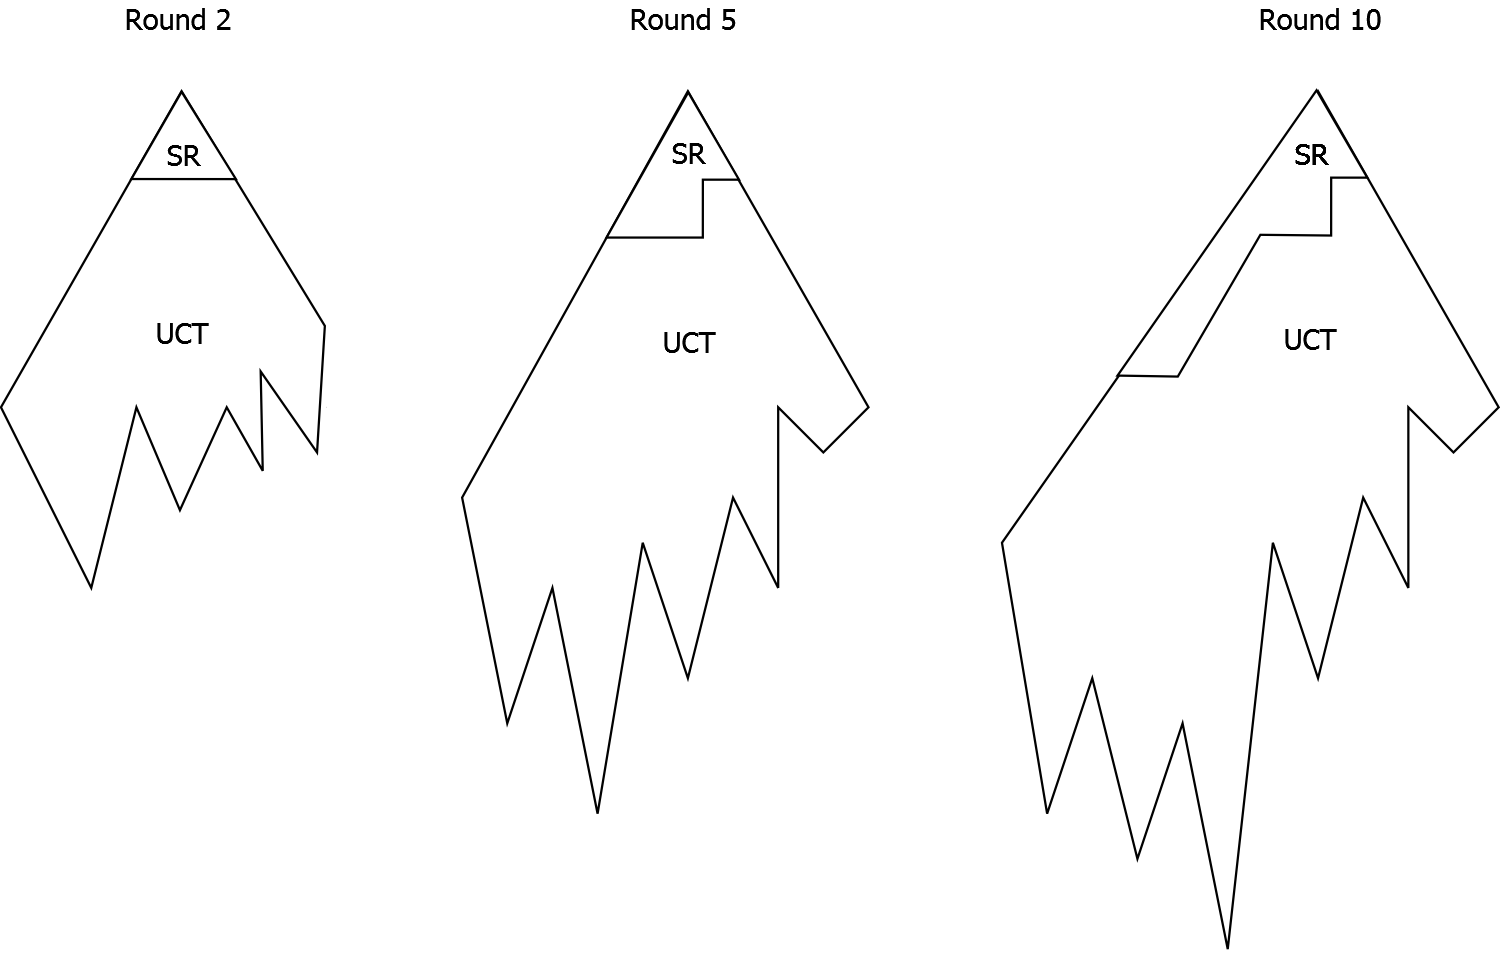
\includegraphics[width=.8\textwidth]{img/H-MCTS.png}
	\caption{Example progression of H-MCTS. In the top part of the tree (SR), simple regret is minimized, in the lower part UCT minimizes cumulative regret. The rounds represent the Sequential Halving round at the root.}
	\label{fig:h-mcts_trees}
\end{figure}

Treating a game tree as a recursive MAB thus reveals different objectives for the distinct plies of the tree. At the root, simple regret should be as low as possible, since the recommendation of the algorithm is based on the first ply of the tree. On deeper plies, we want to both sample efficiently, avoiding time wasted on bad options, and back-propagate correct values from leafs to their ancestors. Where the former can be achieved by using selection policies such as Successive Rejects or Sequential Halving, the latter, as discussed in Section~\ref{sec:mcts} is inherently performed by UCT. Intuitively, this leads to the belief that we should only minimize simple regret at the root, and use UCT throughout of the tree, as suggested by \cite{tolpin2012mcts}.
% lanctot-edit: In the next line: I think I see the argument, but I only buy it if max-backprop was used for the SR portion. So I changed "leads" to "could ... lead"
%However, considering that at any ply, based on the MinMax principle, we want to find the \emph{best reply} to the action of the parent. It may also be beneficial to ensure a low simple regret on that particular move. Because this intrinsically leads to an improved evaluation of the parent.
However, considering that at any node, based on the MinMax principle, we want to find the \emph{best reply} to the action of the parent. It may also be beneficial to ensure a low simple regret on that particular move because this could intrinsically lead to an improved evaluation of the parent.

Using a selection policy based on both SHOT and UCT, Hybrid MCTS (H-MCTS) combines simple and cumulative regret minimization in a tunable algorithm. The rationale is based on the results in~\cite{Bubeck11Pure}, which show that given a low sampling budget, UCB empirically realizes lower simple regret. 
% lanctot-edit: not sure why you wrote the opposite way?
%The proposed technique switches from UCT to Sequential Halving whenever the computational budget is above the budget limit $B$.
The proposed technique switches from Sequential Halving to UCT whenever the computational budget is below the budget limit $B$.
Consequently, the search tree is composed of a \emph{simple regret tree} at the root, and \emph{UCT trees} rooted at the leafs of the simple regret tree. As shown in Figure~\ref{fig:h-mcts_trees}, initially the simple regret tree is shallow because the computational budget per node is small. Later, when the budget per node increases due to nodes being removed from selection as per Sequential Halving, the simple regret tree grows deeper. Note that, since the root's children are sorted in descending order, the left part of the simple regret and UCT tree is always the deepest, since it its root is selected the most.

\IncMargin{1em}
\begin{algorithm2e}
\setstretch{1.1}
	\KwIn{node $p$, allocated budget $budget$}
	\KwOut{$t_s$: number of play-outs, $p1$ and $p2$ wins}
	\vspace{0.1cm}
	\func{h-mcts}(node $p$, $budget$):												\;
	\Indp
	\lIf{isLeaf($p$)}{$S\gets$ \func{expand}($p$)}					
	$t_s \gets \tuple{0,0,0}$														\;		
	\If{isTerminal($p$)}{															\label{h-mcts:terminal}
		\func{update} $t_s$, with $budget$ wins and visits							\;
		 \KwRet{$t_s$}
	}
	$b \gets \max{\left(1, \floor[\bigg]{\frac{p.budgetSpent + budget}{s\times\ceil{log_2{|S|}}}}\right)}$ \; \label{h-mcts:budgetlimit}
	\If{not isRoot($p$) \textbf{and} $b < B $}{
		\For{i=0 \emph{\KwTo} budget}{
			$\tuple{v, w_1, w_2}_i \gets$ \func{uct}($p$)							\;
			\func{update} $p, t_s$ with $\tuple{v, w_1,w_2}_i$							\;
		}
		\KwRet{$t_s$}
	}
	$b_u, k \gets 0$\; $S_0 \gets S$\; $s \gets |S|$								\;
	\Repeat{$b_u \geq budget$ \textbf{or} $s < 2$} {								\label{h-mcts:shot}
		\For{i=0 \emph{\KwTo} s}{
			$n_i \gets$ node $n$ at rank $i$ of $S_k$								\;			
			\If{$b > n_i.visits$} {
				$b_i \gets b - n_i.visits$											\;
				\lIf{$i = 0$ \textbf{and} $s = 2$} { $b_i \gets \max{(b_i, budget - b_u - (b - n_1.visits))}$ }
				$b_i \gets \min{(b_i, budget - b_u)}$								\;
				$\tuple{v, w_1, w_2}_i \gets$ \func{h-mcts}($n_i$, $b_i$)			\;
				\func{update} $p, b_u$, and $t_s$ with $\tuple{v, w_1, w_2}_i$		\; \label{h-mcts:update}
			}
			break if $b_u \geq budget$												\;
		}
		$s \gets s - \floor{\nicefrac{s}{2}}$, $k \gets k + 1$							\;
		$S_{k} \gets$ $S_{k-1}$, with the first $s$ elements sorted in descending order	\;	\label{h-mcts:sort}
		$b \gets b + \max{\left(1, \floor[\bigg]{\frac{p.budgetSpent + budget}{s\times\ceil{log_2{|S|}}}}\right)}$\;
	}
	\func{update} $p.budgetSpent$ with $b_u$										\;
	\Indm
	\KwRet{$t_s$}
  \caption{Hybrid Monte-Carlo Tree Search (H-MCTS). \label{alg:h-mcts}}
\end{algorithm2e}
\DecMargin{1em}

H-MCTS is outlined in Algorithm~\ref{alg:h-mcts}. Similar to UCT and SHOT, on line~\ref{h-mcts:terminal} terminal conditions are handled. Followed by the main feature of the algorithm on line~\ref{h-mcts:budgetlimit} where the initial simulation budget $b$ for each child of the current node is computed. Based on $b$, a decision is made whether to progress into the UCT tree if $b<B$ or, if $b \geq B$ to continue with SHOT. Note that, the $b<B$ check is overridden at the root, since only one cycle is initiated there. Assuming the allocated budget is large, at the root simple regret minimization is preferred over cumulative regret minimization. From line~\ref{h-mcts:shot} the algorithm is similar to the Sequential Halving portion of SHOT. As in SHOT, because multiple play-outs are back-propagated in a single descent from root to leaf, the algorithm returns a tuple $t_s$, which contains: 1) the number of visits $v$, and 2) the number of wins per player $w_1$ and $w_2$. On line~\ref{h-mcts:update}, the budget used $b_u$ is incremented by $v$ from the results returned by the recursion. Moreover, the current node's statistics are updates, alongside the cumulative tuple $t_s$, which will be returned to the node's parent. UCT also maintains a tuple of statistics such that it can return the same $t_s$ to the simple regret tree. For the UCT tree, any implementation can be used, as long as it is adapted to return $t_s$ and update the $budgetSpent$ value alongside the usual node's visit count. Because any UCT node in the tree can be ``converted'' to a simple regret node at any time, when $b>B$ on line~\ref{h-mcts:budgetlimit}. 

Whenever a UCT node is included in the simple regret tree, all its values are maintained. As such, Sequential Halving has an initial estimate of the values of the nodes. Based on the budgeting method of SHOT~\cite{Cazenave14SHOT}, budget is reallocated such that it adheres to Sequential Halving's allocation. Note that, H-MCTS' implementation details differ from SHOT mainly in the manner that repeating cycles are performed.

In the scheme presented, a limit on the available budget determines whether to continue in the simple regret tree. However, other methods, such as a fixed depth limit for the simple regret tree, or a time-partitioned method, can certainly be viable. Though, based on the simple regret theory, pure exploration methods  only provide empirically better simple regret than UCT, given a sufficiently large budget. Given a low budget, UCT with a properly tuned constant should be preferred~\cite{Bubeck11Pure}.

As with MCTS, H-MCTS can be separated in four discrete steps.
\begin{enumerate}
\item \textbf{Budgeting}: A budget is determined for each child. Based on the budget, we enter the UCT tree, or remain in the simple regret tree. If we enter the UCT tree, the four basic MCTS steps apply.
\item \textbf{Selection}: In the simple regret tree, nodes are sampled based on Sequential Halving. Nodes in the simple regret tree are assigned a budget, to be spent in their rooted UCT tree, in which play-outs are initiated.
\item \textbf{Removal}: Based on the results obtained, children are removed from selection. A new Sequential Halving round starts with half of the best children from the previous round. If the budget is spent, the currently accumulated results are back-propagated.
\item \textbf{Back-propagation}: Since H-MCTS is performed depth-first, the final result is only available after all budget is spent. This results in simultaneous back-propagation of numerous results in the simple regret tree.
\end{enumerate}
Note that, in this case Sequential Halving is presented as the simple regret algorithm. However, it is certainly possible to replace it with any other algorithm such as Successive Rejects, or any other form of sequential reduction.

H-MCTS shares its disadvantage of not being able to return a recommendation at any-time with SHOT. It must know its exact computational budget beforehand. However, it does make use of the fact that UCT is any-time. Suppose a node was selected and expanded by H-MCTS, then at each time in the simple regret tree, nodes have an appropriate value based on the results back-propagated by UCT. Thus, when SHOT finishes a round by sorting the nodes by their accumulated values on line~\ref{h-mcts:sort}, UCT's any-time property ensures nodes have a representative value.

To a lesser extent, H-MCTS shares the speed benefits of SHOT. However, because a large part of the search is performed by UCT, H-MCTS spends more time in the tree than SHOT overall. However, given a lower budget limit $B$, H-MCTS can be made to run faster by increasing the ratio of the simple regret tree related to the UCT tree.

In the form presented in Algorithm~\ref{alg:h-mcts}, H-MCTS cannot solve proven wins or losses in the simple regret tree. Although we can employ the MCTS-Solver proposed by Winands~\emph{et al.}~\cite{Winands2008} in the UCT tree, this solver is to be adapted to be able to solve nodes in the SHOT portion of the algorithm. Such a mechanism has been developed and will be presented in an upcoming master thesis by the first author of this paper.

\section{Experiments and Results}
\label{sec:exp_res}
In this section we show the results of the experiments performed on six two-player games. H-MCTS and the games were implemented in two different engines. Amazons, Breakthrough, NoGo and Pentalath are implemented in a Java based engine. Ataxx and AtariGo are implemented in a \emph{C++} based engine.
\begin{itemize}
\item \emph{Amazons} is played on a 10$\times$10 chessboard. Players each have four Amazons that move as queens in chess. Moves consist of two parts, movement, and shooting an arrow to block a square on the board. The last player to move wins the game.
\item \emph{AtariGo}, or first-capture Go, is a variant of Go where the first player to capture any stones wins. The experiments are performed on a 9$\times$9 board.
\item \emph{Ataxx} is a game similar to Reversi. Played on a square board, players start with two stones each placed in an opposite corner. Captures are performed by moving a stone alongside an opponent's on the board. In the variant used in this paper, jumps are not allowed. The game ends when all squares are filled, or when a player has no remaining stones. The player with the most stones wins.  The experiments are performed on a 7$\times$7 board.
\item \emph{Breakthrough} is played on an 8$\times$8 board. Players start with 16 pawns. The goal is to move one of them to the opponent's side.
\item \emph{NoGo} is a combinatorial game based on Go. Captures are forbidden and the first player unable to play due to this rule, loses. The experiments are performed on a 9$\times$9 board.
\item \emph{Pentalath} is a connection game played on a hexagonal board. The goal is to place 5 pieces in a row. Pieces can be captured by fully surrounding an opponent's set of pieces.
\end{itemize}

All games use a uniform random selection policy during the play-outs, unless otherwise stated. The $C$ constant, used by UCT (Equation \ref{eq:uct}) was optimized for each game and was not re-optimized for H-MCTS, unless otherwise stated both UCT and H-MCTS use the same $C$ constant. The budget limit $B$ which determines the switching point between the simple and UCT trees, was optimized for each game independently using a range between $10$ and $90$, and interval $20$.

Because H-MCTS cannot be terminated any-time we present only results for a fixed number of simulations. In each experiment, both players are allocated a budget of both 10,000 and 25,000 play-outs.
\newpage
\subsection{Results}
\label{subsec:results}

For each table, the results are shown with respect to the first algorithm mentioned in the captions, along with a 95\% confidence interval. For each experiment, the players' seats were swapped such that 50\% of the games are played as the first player, and 50\% as the second, to ensure no first-player or second-player bias. 

\begin{table}[ht]
\centering
\tabcolsep=0.3cm
\scalebox{0.91}{
\begin{tabular}{rlll}
\hline
\multicolumn{2}{c|}{} & \multicolumn{1}{c}{\textbf{10,000}} & \multicolumn{1}{c}{\textbf{25,000}} \\ 
\textbf{Game} & \multicolumn{1}{c|}{\textbf{$B$}} & \multicolumn{1}{c}{\textbf{play-outs}} & \multicolumn{1}{c}{\textbf{play-outs}} \\ [1mm] 
\cline{1-4}
\multicolumn{2}{c|}{} \\ [-3mm]
Amazons &\multicolumn{1}{l|}{50}			    	& {\bf{65.2}} $\pm$ 3.0 		& {\bf{62.0}} $\pm$ 3.0 		\\ [.5mm] 
AtariGo 9$\times$9 &\multicolumn{1}{l|}{30} 		& 50.0 $\pm$ 3.0 				& {\bf{57.5}} $\pm$ 3.1 	\\ [.5mm] 
Ataxx 7$\times$7 &\multicolumn{1}{l|}{30} 			& {\bf{54.5}} $\pm$ 3.1			& {\bf{56.0}} $\pm$ 3.1 		\\ [.5mm] 
Breakthrough 8$\times$8 &\multicolumn{1}{l|}{70}	& {\bf{53.2}} $\pm$ 3.1			& 50.4 $\pm$ 3.1 				\\ [.5mm] 
NoGo 9$\times$9 &\multicolumn{1}{l|}{30} 			& 52.4 $\pm$ 3.1				& 48.8 $\pm$ 3.1 				\\ [.5mm] 
Pentalath &\multicolumn{1}{l|}{30} 		  			& 46.7 $\pm$ 3.1				& {\bf{54.7}} $\pm$ 3.1			\\ [.5mm] 
\hline
\end{tabular}
}
\vspace{3mm}
{\caption{H-MCTS vs. UCT with random play-outs, 1,000 games} \label{tab:uct_hmcts}}
\end{table}

Table~\ref{tab:uct_hmcts} shows results of the matches played by H-MCTS against a standard UCT player. H-MCTS performs best in Amazons, Ataxx, and AtariGo. For Amazons this is in part due to the high branching factor. Since UCT cannot explore and exploit all options in time, Sequential Halving ensures that only a limited subset of the large action-space is under consideration. For the other games we see no significant improvement over UCT. This may be due to the fact that these games have quite narrow winning-lines, and a more exploiting algorithm applies better by identifying and exploiting them fast. However, it is also possible that H-MCTS requires separate tuning of its UCT $C$ constant in these games. This optimization was performed for Ataxx and AtariGo, which resulted in winning rates for H-MCTS of {\bf{57.6\%}} $\pm$ 3.1, and {\bf{58.1\%}} $\pm$ 3.1 in Ataxx, and {\bf{61.7}} $\pm$ 3.0, and {\bf{66.6}} $\pm$ 3.0 in AtariGo, for 10,000 and 25,000 play-outs respectively. Providing evidence from two  of the games that performance can be improved by separately tuning the $C$ constant in H-MCTS.

\begin{table}[ht]
\centering
\tabcolsep=0.3cm
\scalebox{0.91}{
\begin{tabular}{rlll}
\hline
\multicolumn{2}{c|}{} & \multicolumn{1}{c}{\textbf{10,000}} & \multicolumn{1}{c}{\textbf{25,000}} \\ 
\textbf{Game} & \multicolumn{1}{c|}{\textbf{$B$}} & \multicolumn{1}{c}{\textbf{play-outs}} & \multicolumn{1}{c}{\textbf{play-outs}} \\ [1mm] 
\cline{1-4}
\multicolumn{2}{c|}{} \\ [-3mm]
Amazons &\multicolumn{1}{l|}{50}			    	& 51.2 $\pm$ 3.1 			& {\bf{55.4}} $\pm$ 3.1 	\\ [.5mm] 
AtariGo 9$\times$9 &\multicolumn{1}{l|}{30} 		& 50.0 $\pm$ 3.1 			& {\bf{57.5}} $\pm$ 3.1		\\ [.5mm] 
Ataxx 7$\times$7 &\multicolumn{1}{l|}{30} 			& {\bf{54.5}} $\pm$ 3.1		& {\bf{56.0}} $\pm$ 3.1 	\\ [.5mm] 
Breakthrough 8$\times$8 &\multicolumn{1}{l|}{70}	& {\bf{68.4}} $\pm$ 2.9  	& {\bf{84.0}} $\pm$ 2.3 	\\ [.5mm] 
NoGo 9$\times$9 &\multicolumn{1}{l|}{30} 			& {\bf{56.3}} $\pm$ 3.1 	& {\bf{55.5}} $\pm$ 3.1 	\\ [.5mm] 
Pentalath &\multicolumn{1}{l|}{30} 		  			& {\bf{62.1}} $\pm$ 3.0		& {\bf{78.3}} $\pm$ 2.6  	\\ [.5mm] 
\hline
\end{tabular}
}
\vspace{3mm}
{\caption{H-MCTS vs. SHOT with random play-outs, 1,000 games} \label{tab:shot_hmcts}}
\end{table}
\begin{table}[ht]
\centering
\tabcolsep=0.45cm
\scalebox{0.91}{
\begin{tabular}{r|ll}
\hline
 & \multicolumn{1}{c}{\textbf{10,000}} & \multicolumn{1}{c}{\textbf{25,000}} \\ 
\textbf{Game} & \multicolumn{1}{c}{\textbf{play-outs}} & \multicolumn{1}{c}{\textbf{play-outs}} \\ [1mm] 
\cline{1-3}
\multicolumn{1}{c|}{} & \multicolumn{2}{c}{} \\ [-3mm]
Amazons 			    	& {\bf{60.2}} $\pm$ 3.0 	& {\bf{55.2}} $\pm$ 3.1 	\\ [.5mm] 
AtariGo 9$\times$9  		& {\bf{53.8}} $\pm$ 3.1 	& {\bf{55.7}} $\pm$ 3.1 	\\ [.5mm] 
Ataxx 7$\times$7  			& 46.7 $\pm$ 3.1			& 40.8 $\pm$ 3.1 			\\ [.5mm] 
Breakthrough 8$\times$8 	& 31.2 $\pm$ 3.1			& 16.4 $\pm$ 2.3 			\\ [.5mm] 
NoGo 9$\times$9  			& 44.7 $\pm$ 3.1 			& 41.4 $\pm$ 3.1 			\\ [.5mm] 
Pentalath 		  			& 33.7 $\pm$ 3.0 			& 22.8 $\pm$ 2.6 			\\ [.5mm] 
\hline
\end{tabular}
}
\vspace{3mm}
{\caption{SHOT vs. UCT with random play-outs, 1,000 games} \label{tab:uct_shot}}
\end{table}

To compare the effect of the hybrid method effectively, we show the results of matches played by H-MCTS against SHOT in Table~\ref{tab:shot_hmcts}. H-MCTS shows significant improvement in 10 of the 12 cases. Note that, we make no use of the speed benefits of either technique in these experiments. This gives evidence for the claim that H-MCTS makes use of UCT's any-time property to provide good utility estimates in the simple regret tree, values back-propagated by UCT may be more effective than those back-propagated by using Sequential Halving throughout the tree. 
As a benchmark, SHOT played 1,000 matches against UCT per game in Table~\ref{tab:uct_shot}. SHOT performs best against H-MCTS and UCT in the games with the highest branching factors, Amazons, AtariGo and to a lesser extent, NoGo. This reinforces the evidence that Sequential Halving is best applied in games with high branching factors. In the games with narrow winning-lines such as Breakthrough and Pentalath, SHOT's performance declines against UCT.
\begin{table}[ht]
\centering
\tabcolsep=0.3cm
\scalebox{0.9}{
\begin{tabular}{rlcc}
\hline
\multicolumn{2}{c|}{} & \multicolumn{1}{c}{\textbf{10,000}} & \multicolumn{1}{c}{\textbf{25,000}} \\ 
\textbf{Game} & \multicolumn{1}{c|}{\textbf{$B$}} & \multicolumn{1}{c}{\textbf{play-outs}} & \multicolumn{1}{c}{\textbf{play-outs}} \\ [1mm] 
\cline{1-4}
\multicolumn{2}{c|}{} \\ [-3mm]
\multicolumn{2}{c|}{} & \multicolumn{2}{c}{\textbf{Heuristic play-outs (no solver)}} \\ [1mm]
\multicolumn{2}{c|}{} \\ [-4mm]
Breakthrough 8$\times$8 &\multicolumn{1}{l|}{70}	& 50.4 $\pm$ 3.1				& {\bf{56.6}} $\pm$ 3.1 	\\ [.5mm]
\multicolumn{2}{c|}{} \\ [-4mm]
\multicolumn{2}{c|}{} & \multicolumn{2}{c}{\textbf{H-MCTS Solver}} 					\\ [1mm]
\cline{1-4}
\multicolumn{2}{c|}{} \\ [-4mm]
Amazons &\multicolumn{1}{l|}{50}			    	& {\bf{65.2}} $\pm$ 3.0 		& {\bf{64.0}} $\pm$ 3.0 	\\ [.5mm] 
Breakthrough 8$\times$8 &\multicolumn{1}{l|}{70}	& {\bf{56.7}} $\pm$ 3.1		& {\bf{61.3}} $\pm$ 3.0 	\\ [.5mm]
NoGo 9$\times$9 &\multicolumn{1}{l|}{30} 			& 50.5 $\pm$ 3.1			& 50.6 $\pm$ 3.1 			\\ [.5mm] 
Pentalath &\multicolumn{1}{l|}{70} 		  			& 46.7 $\pm$ 3.1			& 52.3 $\pm$ 3.1 			\\ [.5mm] 
\hline
\end{tabular}
}
\vspace{3mm}
%lanctot-edit
%{\caption{H-MCTS vs. UCT with heuristic play-outs and solver, 1,000 games} \label{tab:uct_hmcts-s-h}}
{\caption{H-MCTS vs. UCT with heuristic play-outs, with/without solver, 1,000 games} \label{tab:uct_hmcts-s-h}}
\end{table}

In Table~\ref{tab:uct_hmcts-s-h}, an informed play-out policy is used to select moves for Breakthrough. The policy selects over a non-uniform move distribution based on the properties of the moves, and (anti-)decisive moves are always played when available. UCT with these play-out policies enabled wins approximately 78\% of games against UCT with random play-outs. H-MCTS benefits more from the informed play-outs than UCT in Breakthrough. The second part of Table~\ref{tab:uct_hmcts-s-h} shows results for matches played between the H-MCTS-Solver and the MCTS-Solver. Breakthrough employs the heuristic play-out policy, for which we see a significant boost in performance, proportional to the allocated budget. Overall, the results show some improvement over Table~\ref{tab:uct_hmcts} in Pentalath and NoGo with 25,000 play-outs, although the difference is not sufficient to conclude that the Solver performs better in H-MCTS than in UCT in these games with the same $C$ constant.

\section{Conclusion and Future Research}
\label{sec:concl}
In this paper an MCTS technique is presented based on the results of research in regret theory. The conclusions of the research performed in \cite{Bubeck11Pure} were interpreted into the form of a Hybrid MCTS technique (H-MCTS). Based on minimizing simple regret near the root, where the overall budget is high, and cumulative regret deeper in the tree~\cite{tolpin2012mcts}. However, based on available budget H-MCTS' simple regret tree can expand deeper to provide both better bounds on simple regret on the best-replies of rooted subtrees. The simple regret tree is traversed in a similar manner as SHOT~\cite{Cazenave14SHOT}.

Results show that in different two-player games, H-MCTS performs either better than, or on par with UCT. In Amazons, Ataxx, and AtariGo H-MCTS outperforms UCT up to 66.6\%. Moreover, H-MCTS performed better than SHOT given the same allocation of play-outs in 10 out of 12 experiments performed.

In an upcoming master's thesis, two enhancements for H-MCTS will be proposed. First, the H-MCTS Solver, based on the MCTS-Solver~\cite{Winands2008}, in which solved nodes in both the simple regret, and UCT tree can be proven. Second, an enhancement providing improved selection in the simple regret tree, based on comparing the lower confidence bound of the best child to the upper confidence bound of the others. This enhancement reduces time misspent on nodes that cannot improve upon the current estimated best one.

%lanctot-edit: This point is not just about theory. There are theoretical bounds on simple regret and measurable/observed simple regret (also called average error in the BRUE paper or simply just Regret in the MCMS paper) in practice. These are two separate things; we showed neither. I think you should show the latter in your thesis. 
%Note that, although the hybrid technique is founded on theoretical work in both the MAB context, and MCTS, we have not shown that it provides better bounds on simple regret compared to UCT. This is work for future research. In order to show that H-MCTS provides a better bound on simple regret, the technique should be validated in smaller, proven games for which the game-theoretic value of each action is known.
Note that, although the hybrid technique is founded on theoretical work in both the MAB context, and MCTS, we have not shown that it provides better bounds on simple regret compared to UCT. This is work for future research. In order to show that H-MCTS exhibits lower simple regret in practice, the technique should be validated in smaller, proven games for which the game-theoretic value of each action is known. Moreover, investigation is required regarding the effects of the budget limit $B$ in relation to the total allocated number of play-outs, and the interrelation between H-MCTS' $B$, and UCT's $C$ constant. In the experiments presented in this paper, both were fixed per game, rather than per experiment. Finally, the speed benefits of H-MCTS, combined with parallelization of the algorithm is open to investigation. H-MCTS can be parallelized efficiently by dividing budgets in the simple regret tree over multiple threads~\cite{Cazenave14SHOT}.

\subsection*{Acknowledgments} 
This work is partially funded by the Netherlands Organisation for Scientific Research (NWO) (NWO) in the framework of the project Go4Nature, grant number 612.000.938.

\bibliographystyle{splncs03}
\bibliography{h-mcts}
\end{document}
